If we are talking about dynamic programming most of the times it is an optimization of a solution that use recursion. As we know most of the times use recursion results in an exponential complexity in time so if we find a way to use dynamic programming we can reduce this complexity.\\

\paragraph{What is the main idea of use Dynamic programming?}
The idea is very simple, if we can store the result of the subproblems, we do not need to re-calculate this subproblem and it reduces the complexity from exponential to a polynomial. 

\subsection{Examples}
We can use the idea of calculate a factorial number, we know that a factorial number it is the multiplication of all the numbers from 1 to n, for example

\begin{itemize}
    \item { Calculate 2! = 1 * 2 = 2}
    \item { Calculate 3! = 1 * 2 * 3 = 6}
    \item { Calculate 5! = 1 * 2 * 3 * 4 * 5  = 120}
\end{itemize}

But we need to consider some things about factorial numbers
\begin{enumerate}
    \item { 0! = 1 }
    \item { Factorial numbers exist in range of $[0, \infty)$ }
\end{enumerate}

If we know this we can notice that we can get a formula to simplify this:
\[
    factorial( n ) = 
    \begin{cases*}
        1 & if $0 \leq n \leq 1$ \\
        n * factorial(n - 1) & if $n \geq 2$
    \end{cases*}
\]

Now we can solve this problem using a recursive program, it is very simple because we just need to programm the formula 
\begin{lstlisting}
    #include<bits/stdc++.h>

    using namespace std;
    typedef long long int lli;
    
    lli factorial( int n ){
        return n * factorial(n);
    }

    int main(){
        int n;
        cin >> n;
        cout << factorial( n ) << endl;
        return 0;
    }
\end{lstlisting}

If we use the last program we can get the factorial of n, but the complexity of this algorithm is $O(n!)$ so it is awful, but using dynamic programming can we get a better complexity? \\

For me is easier to find a solution using dynamic programming using draws, so I go to make the draw of the recursive calls of the example 5!

\begin{figure}[H]
\begin{center}
    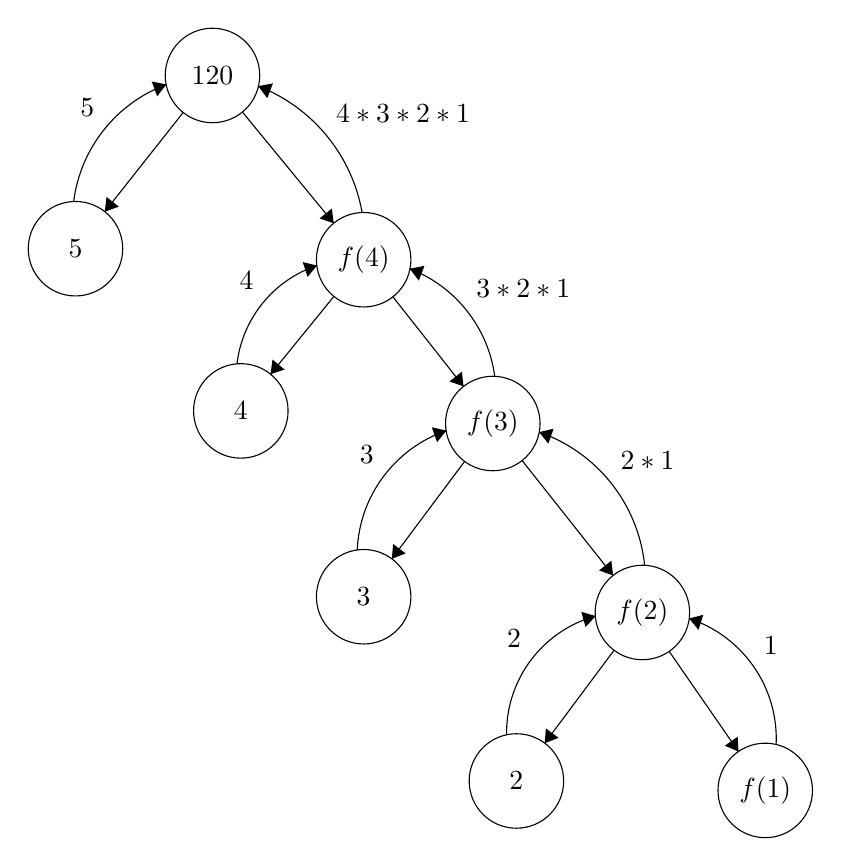
\begin{tikzpicture}[scale=0.2]
    \tikzstyle{every node}+=[inner sep=0pt]
    \draw [black] (30.8,-6.3) circle (3);
    \draw (30.8,-6.3) node {$120$};
    \draw [black] (22.1,-17.3) circle (3);
    \draw (22.1,-17.3) node {$5$};
    \draw [black] (40.4,-18) circle (3);
    \draw (40.4,-18) node {$f(4)$};
    \draw [black] (32.6,-27.6) circle (3);
    \draw (32.6,-27.6) node {$4$};
    \draw [black] (48.6,-28.4) circle (3);
    \draw (48.6,-28.4) node {$f(3)$};
    \draw [black] (40.4,-39.4) circle (3);
    \draw (40.4,-39.4) node {$3$};
    \draw [black] (58.1,-40.4) circle (3);
    \draw (58.1,-40.4) node {$f(2)$};
    \draw [black] (65.9,-51.7) circle (3);
    \draw (65.9,-51.7) node {$f(1)$};
    \draw [black] (50.1,-51.1) circle (3);
    \draw (50.1,-51.1) node {$2$};
    \draw [black] (28.94,-8.65) -- (23.96,-14.95);
    \fill [black] (23.96,-14.95) -- (24.85,-14.63) -- (24.07,-14.01);
    \draw [black] (32.7,-8.62) -- (38.5,-15.68);
    \fill [black] (38.5,-15.68) -- (38.38,-14.75) -- (37.6,-15.38);
    \draw [black] (38.51,-20.33) -- (34.49,-25.27);
    \fill [black] (34.49,-25.27) -- (35.38,-24.97) -- (34.61,-24.34);
    \draw [black] (42.26,-20.36) -- (46.74,-26.04);
    \fill [black] (46.74,-26.04) -- (46.64,-25.11) -- (45.85,-25.73);
    \draw [black] (50.46,-30.75) -- (56.24,-38.05);
    \fill [black] (56.24,-38.05) -- (56.13,-37.11) -- (55.35,-37.73);
    \draw [black] (46.81,-30.81) -- (42.19,-36.99);
    \fill [black] (42.19,-36.99) -- (43.07,-36.65) -- (42.27,-36.05);
    \draw [black] (59.8,-42.87) -- (64.2,-49.23);
    \fill [black] (64.2,-49.23) -- (64.15,-48.29) -- (63.33,-48.86);
    \draw [black] (56.3,-42.8) -- (51.9,-48.7);
    \fill [black] (51.9,-48.7) -- (52.78,-48.36) -- (51.97,-47.76);
    \draw [black] (61.058,-40.782) arc (71.94761:-2.71565:8.032);
    \fill [black] (61.06,-40.78) -- (61.66,-41.5) -- (61.97,-40.55);
    \draw (65.78,-42.5) node [right] {$1$};
    \draw [black] (49.475,-48.185) arc (-179.04361:-254.52464:7.711);
    \fill [black] (55.13,-40.63) -- (54.22,-40.36) -- (54.49,-41.32);
    \draw (50.43,-42.04) node [left] {$2$};
    \draw [black] (51.539,-28.946) arc (70.92086:5.81411:10.037);
    \fill [black] (51.54,-28.95) -- (52.13,-29.68) -- (52.46,-28.73);
    \draw (56.69,-30.78) node [right] {$2*1$};
    \draw [black] (39.992,-36.444) arc (-182.37685:-251.02886:8.395);
    \fill [black] (45.65,-28.85) -- (44.73,-28.64) -- (45.06,-29.59);
    \draw (41.07,-30.38) node [left] {$3$};
    \draw [black] (33.712,-6.98) arc (68.73994:9.99869:10.591);
    \fill [black] (33.71,-6.98) -- (34.28,-7.74) -- (34.64,-6.8);
    \draw (38.62,-8.7) node [right] {$4*3*2*1$};
    \draw [black] (21.983,-14.316) arc (-187.14018:-249.5414:9.158);
    \fill [black] (27.87,-6.87) -- (26.94,-6.68) -- (27.29,-7.62);
    \draw (23.32,-8.35) node [left] {$5$};
    \draw [black] (43.329,-18.572) arc (68.89286:7.61598:8.553);
    \fill [black] (43.33,-18.57) -- (43.9,-19.33) -- (44.26,-18.39);
    \draw (47.53,-19.84) node [right] {$3*2*1$};
    \draw [black] (32.353,-24.63) arc (-186.66238:-251.52534:7.525);
    \fill [black] (37.44,-18.37) -- (36.53,-18.15) -- (36.84,-19.09);
    \draw (33.43,-19.33) node [left] {$4$};
    \end{tikzpicture}
\end{center}
\end{figure}

As we can see we the small problem contains information of the base case has information of the next case and this case has information for the next case and so on, so we do not need to call. Maybe if you need to calculate just once a factorial number it is not necessary to store the information about a factorial number but imagine that you are doing a program that needs a lot of factorial numbers, if we use the recursive algorithm without dynamic programming we need to do for each query $O(n!)$ operations, and that is a lot. So we can store this information and make each query a lot of times and if we already calculated a factorial number we just need to return the information and it is $O(1)$

\begin{lstlisting}
    #include <bits/stdc++.h>

    using namespace std;
    typedef long long int lli;

    vector< lli > factorial_number( 1000 + 1, -1 )
    lli factorial( int n ){

        if( n == 0 || n == 1 ){
            factorial_number[ n ] = 1;
            return factorial_number[ n ]; 
        }
        if( factorial_number[ n ] != -1 )
            return factorial_number[ n ];
        
        factorial_number[ n ] = n * factorial( n - 1 );
        return factorial_number[ n ];
    }

    int main(){
        int t, n;
        cin >> t;
        while( t-- ){
            cin >> n;
            cout << n << "! = " << factorial( n ) << endl;
        }
        return 0;  
    }
\end{lstlisting}

As you can see we have a little bit of code but we make more efficient get a factorial number, from $O(n!)$ complexity to $O(1)$ in the case of we already calculated the number, but we are using more memory in this case $O(n)$ in other words we are using a container which size is the biggest factorial that we already calculated.